% =====================================================================
% PRISMA 2020 — fluxograma em TikZ (TEMPLATE)
% Preencha os XX (e os <...>) com seus números/motivos.
% Compilar: Overleaf (cole e Recompile) ou  pdflatex prisma_flow_template.tex
% Guia completo: ver README.md nesta pasta.
% =====================================================================
\documentclass[12pt]{article}
\usepackage[utf8]{inputenc}
\usepackage[T1]{fontenc}
\usepackage[english]{babel}
\usepackage{geometry}
\geometry{a4paper, margin=0.6in, portrait}
\usepackage{amsmath}
\usepackage{xcolor}

% --- Custom PRISMA 2020 Color Palette ---
\definecolor{prisma-yellow}{HTML}{FFBD00}
\definecolor{prisma-blue}{HTML}{92B4D8}
\definecolor{headergray}{HTML}{F2F3F4}
\definecolor{navyblue}{HTML}{000080}

\usepackage{tikz}
\usetikzlibrary{arrows.meta, positioning, calc}

\begin{document}

\begin{figure}[htbp]
    \centering
    \resizebox{0.95\linewidth}{!}{
        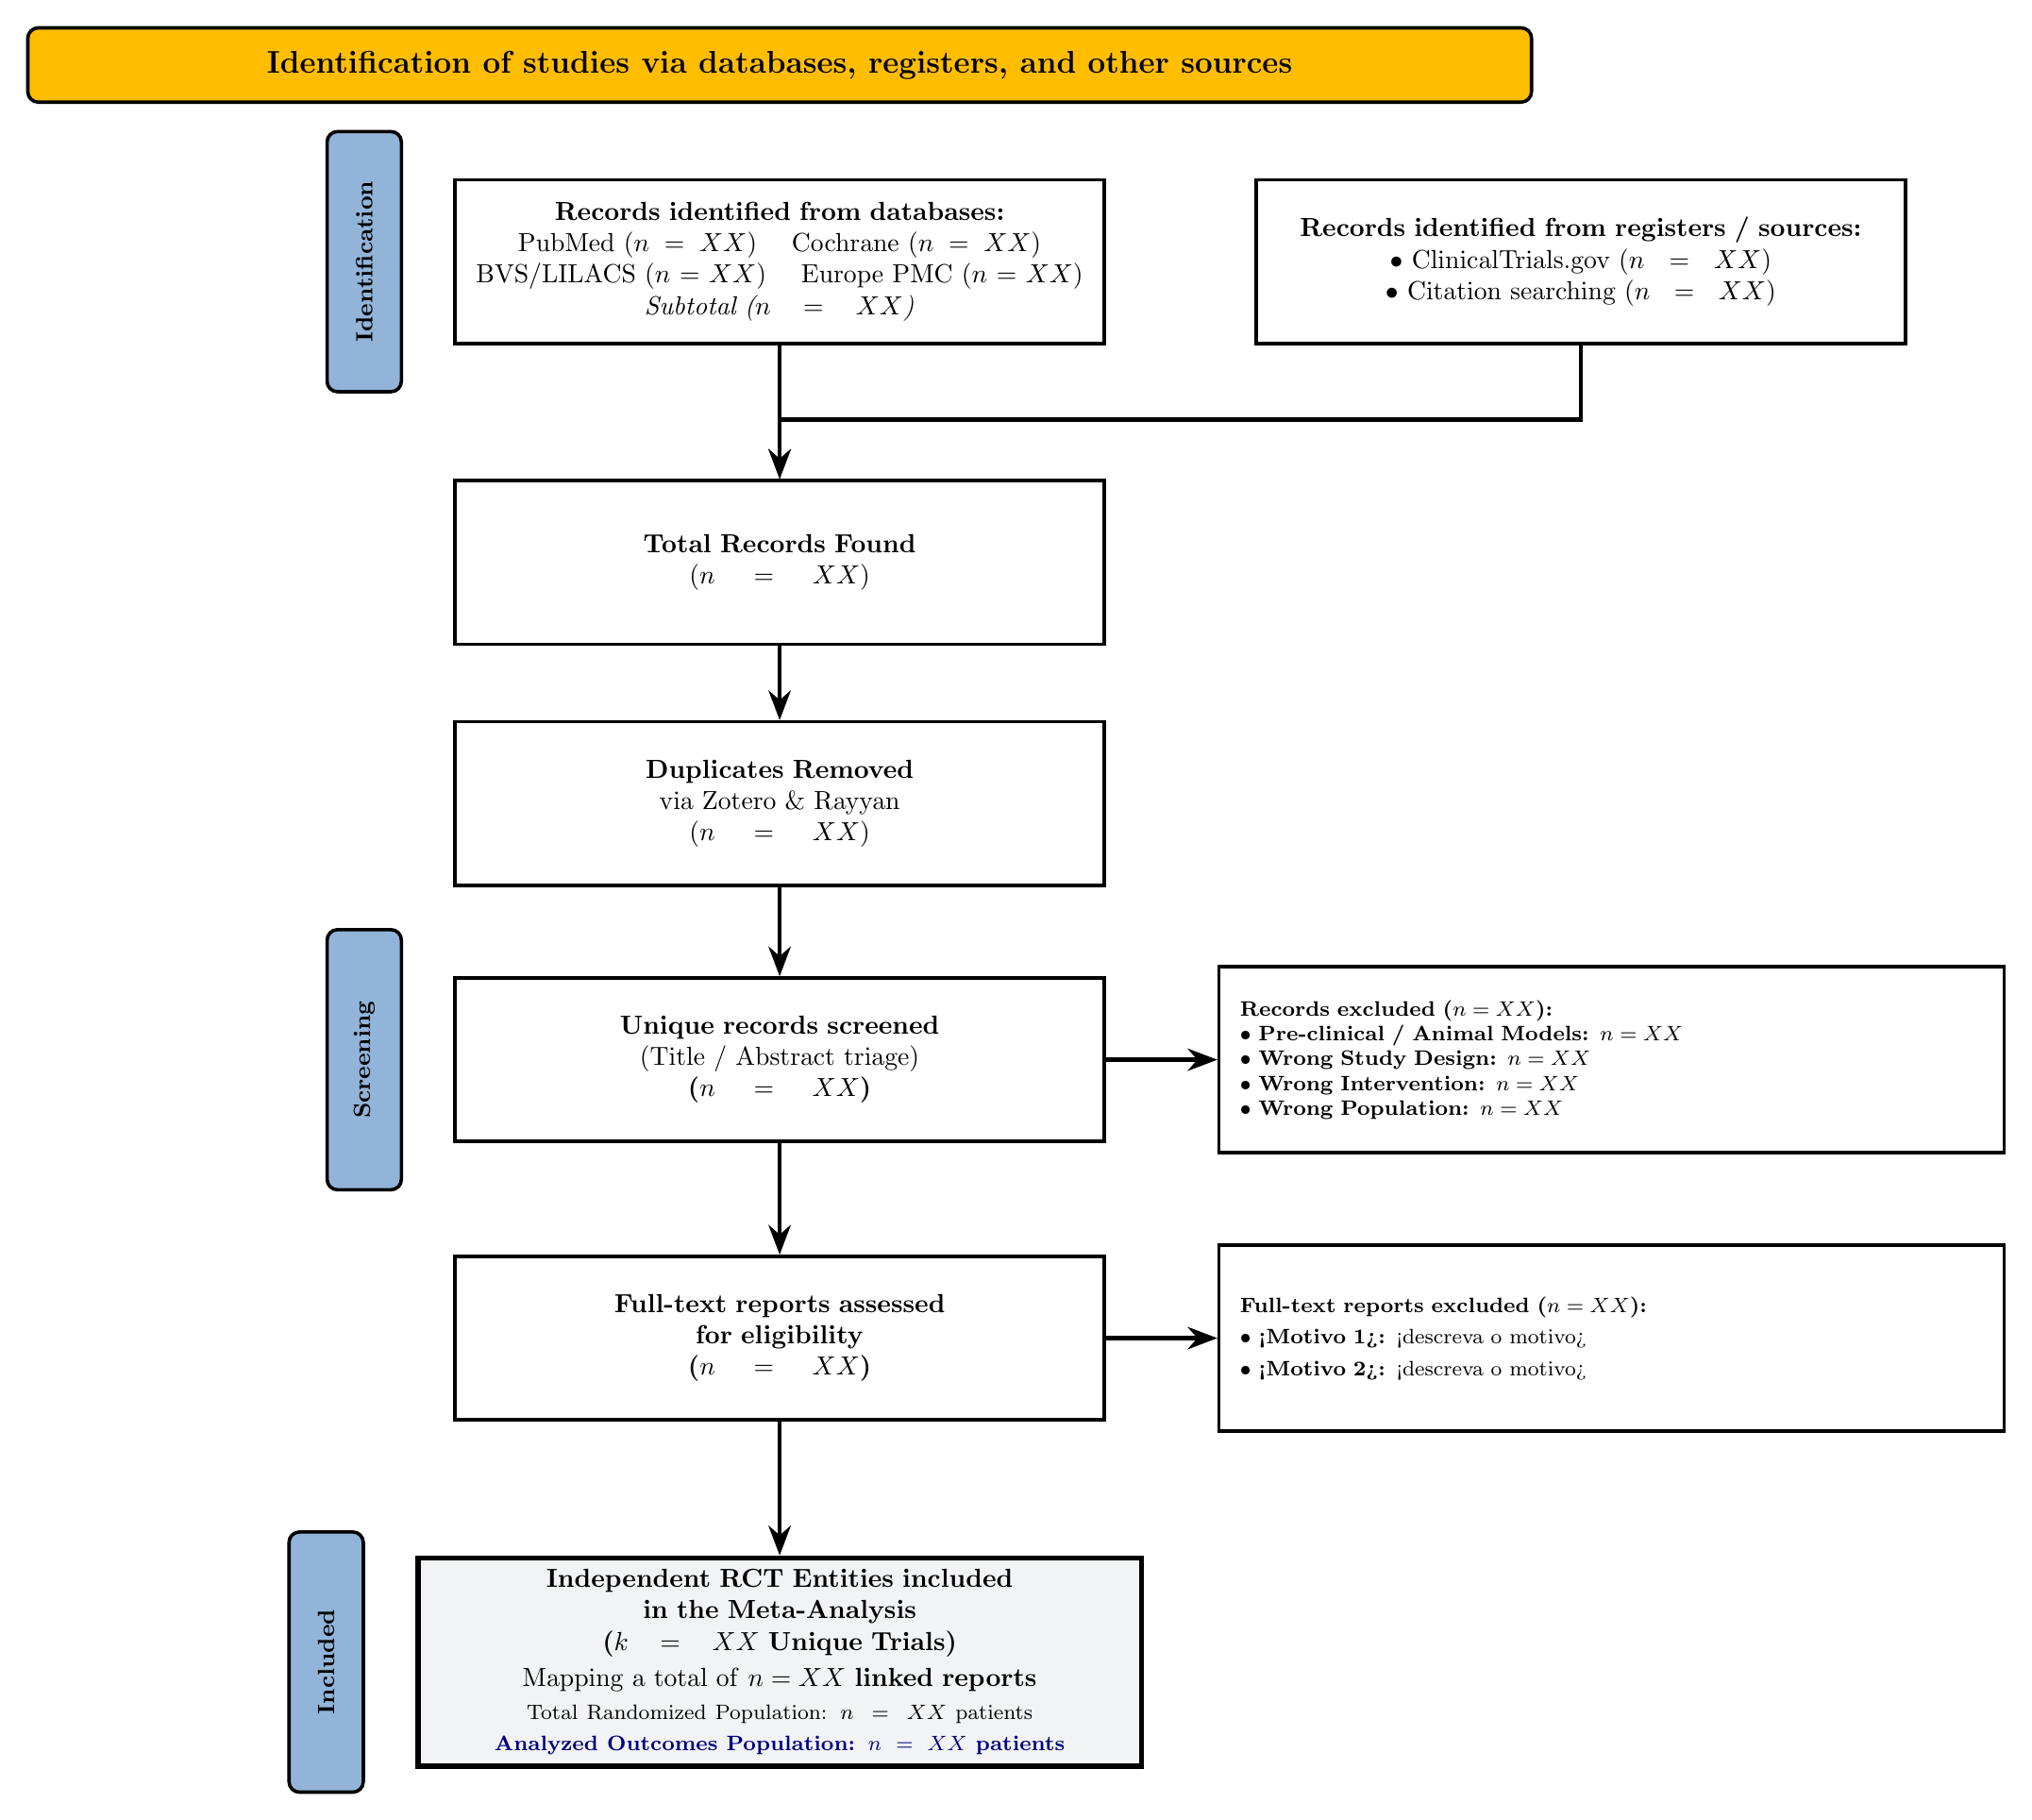
\begin{tikzpicture}[
            node distance=1.0cm and 1.2cm,
            every node/.style={font=\sffamily, line width=1.3pt},
            titlebox/.style={rectangle, draw, fill=prisma-yellow, text width=20cm, minimum height=1.0cm, align=center, font=\bfseries\large, rounded corners=4pt},
            mainbox/.style={rectangle, draw, fill=white, text width=8.5cm, minimum height=2.2cm, align=center, font=\normalsize},
            sidebox/.style={rectangle, draw, fill=white, text width=10.0cm, minimum height=2.5cm, align=left, font=\footnotesize, inner sep=8pt},
            labelbox/.style={rectangle, draw, fill=prisma-blue, minimum width=3.5cm, minimum height=1.0cm, text centered, font=\bfseries\small, rounded corners=4pt, rotate=90, anchor=center},
            arrow/.style={-{Stealth[length=4mm]}, line width=1.6pt}
        ]

        % --- 1. HEADER ---
        \node[titlebox] (htitle) {Identification of studies via databases, registers, and other sources};

        % --- 2. IDENTIFICATION STAGE ---
        \node[mainbox, below=1.0cm of htitle] (db) {
            \textbf{Records identified from databases:}\\
            PubMed ($n = XX$) \quad Cochrane ($n = XX$)\\           % <-- nº por base
            BVS/LILACS ($n = XX$) \quad Europe PMC ($n = XX$)\\
            \textit{Subtotal ($n = XX$)}                            % <-- soma das bases
        };

        \node[mainbox, right=2.0cm of db] (other) {
            \textbf{Records identified from registers / sources:}\\
            $\bullet$ ClinicalTrials.gov ($n = XX$)\\               % <-- registros
            $\bullet$ Citation searching ($n = XX$)
        };

        \node[mainbox, below=1.8cm of db] (tot) {
            \textbf{Total Records Found}\\
            ($n = XX$)                                              % <-- total identificado
        };

        \node[mainbox, below=1.0cm of tot] (dup) {
            \textbf{Duplicates Removed}\\
            via Zotero \& Rayyan\\
            ($n = XX$)                                              % <-- duplicatas
        };

        \node[labelbox] at ($(db.west)-(1.2,0)$) (l_id) {Identification};

        % --- 3. SCREENING STAGE ---
        \node[mainbox, below=1.2cm of dup] (scr) {
            \textbf{Unique records screened}\\
            (Title / Abstract triage)\\
            \textbf{($n = XX$)}                                     % <-- triados (total - duplicatas)
        };

        \node[sidebox, right=1.5cm of scr] (exc) {
            \textbf{Records excluded ($n = XX$):}\\                 % <-- total excluído na triagem
            $\bullet$ \textbf{Pre-clinical / Animal Models:} $n = XX$\\
            $\bullet$ \textbf{Wrong Study Design:} $n = XX$\\
            $\bullet$ \textbf{Wrong Intervention:} $n = XX$\\
            $\bullet$ \textbf{Wrong Population:} $n = XX$
        };

        % --- 4. ELIGIBILITY STAGE ---
        \node[mainbox, below=1.5cm of scr] (elg) {
            \textbf{Full-text reports assessed}\\
            \textbf{for eligibility}\\
            \textbf{($n = XX$)}                                     % <-- textos completos avaliados
        };

        \node[sidebox, right=1.5cm of elg] (reasons) {
            \textbf{Full-text reports excluded ($n = XX$):}\\       % <-- textos completos excluídos
            \vspace*{0.3em}
            $\bullet$ \textbf{<Motivo 1>:} <descreva o motivo> \\
            \vspace*{0.3em}
            $\bullet$ \textbf{<Motivo 2>:} <descreva o motivo>
        };

        \node[labelbox] at ($(scr.west)-(1.2,0)$) (l_scr) {Screening};

        % --- 5. INCLUDED STAGE ---
        \node[mainbox, below=1.8cm of elg, text width=9.5cm, minimum height=2.8cm, line width=2.0pt, fill=headergray] (inc) {
            \textbf{Independent RCT Entities included}\\
            \textbf{in the Meta-Analysis}\\
            \textbf{($k = XX$ Unique Trials)}\\                     % <-- nº de entidades/ensaios
            \vspace*{0.2em}
            \text{Mapping a total of \textbf{$n = XX$ linked reports}} \\  % <-- relatórios vinculados
            \vspace*{0.3em}
            \footnotesize
            Total Randomized Population: $n = XX$ patients\\        % <-- randomizados
            \textbf{\textcolor{navyblue}{Analyzed Outcomes Population: $n = XX$ patients}}  % <-- analisados
        };

        \node[labelbox] at ($(inc.west)-(1.2,0)$) (l_inc) {Included};

        % --- ROUTING ARROWS ---
        \draw[arrow] (db.south) -- (tot.north);
        \draw[arrow] (other.south) -- ++(0,-1.0cm) -| (tot.north);
        \draw[arrow] (tot.south) -- (dup.north);
        \draw[arrow] (dup.south) -- (scr.north);
        \draw[arrow] (scr.east) -- (exc.west);
        \draw[arrow] (scr.south) -- (elg.north);
        \draw[arrow] (elg.east) -- (reasons.west);
        \draw[arrow] (elg.south) -- (inc.north);

        \end{tikzpicture}
    }
\end{figure}

\end{document}
